\documentclass[11pt]{article}


\usepackage{titlesec}
\usepackage{graphicx}
\usepackage{subcaption}
\usepackage{float}
\usepackage[bottom]{footmisc}
\usepackage[hidelinks]{hyperref}


\setlength{\parindent}{1.0em}
\setlength{\parskip}{1.0em}
\setlength{\emergencystretch}{5.0em}
\titlespacing*{\section}{0em}{3.5em}{1.5em}
\setcounter{tocdepth}{1}
\renewcommand{\contentsname}{Contenidos}
\hypersetup{
	linktoc=all
}


\title{\Huge Software en formato fuente}
\author{Eugenia Damonte, Ariel Fideleff y Mart\'in Go\~ni}
\date{}


\begin{document}
	\pagenumbering{gobble}
	\maketitle
	\newpage
	\tableofcontents
	\newpage
	\pagenumbering{arabic}
	
	
	\section{Configuraci\'on previa}
		Antes de comenzar a resolver los ejercicios configur\'e \texttt{vim} para editar archivos en C. Lo primero que hice fue configurar \texttt{vim}, para hacer esto abr\'i el archivo \texttt{\textasciitilde/.vimrc} que es el archivo de configuraci\'on de \texttt{vim}. Esaba vac\'io y le a\~nad\'i dos l\'ineas \texttt{set nocop} y \texttt{filetype plugin on}. Lo que hace el primer comando es desactivar el modo de compatibilidad. Este hace que algunas de las funciones de \texttt{vim} sean deshabilitadas o modificadas para que se comporte de manera similar a \texttt{vi}, el antecesor de \texttt{vim}. La segunda permite utlizar el plugin \texttt{filetype}.
		
		Luego para asegurarme de tener todos los paquetes de \texttt{vim} utlic\'e los comandos \texttt{sudo apt-get install vim-gui-common} y \texttt{sudo apt-get install vim-runtime}. El primer paquete tuvo que instalarse demorando varios minutos por la velocidad de descarga abismal de los repositorios. El segundo, por el otro lado ya estaba instalado.
		
		Finalmente cre\'e el archivo de configuraci\'on para los archivos con extensi\'on \texttt{.c}, llamado \texttt{c.vim}. Para poder crearlo primero tuve que crear la carpeta \texttt{\textasciitilde/.vim/ftplugin}, que es donde se ponen los archivos de configuraci\'on. Luego abr\'i el mismo con vim y escrib\'i las configuraciones que quer\'ia usar.
		\begin{figure}[H]
			\centering
			\begin{subfigure}[b!]{0.7\linewidth}
				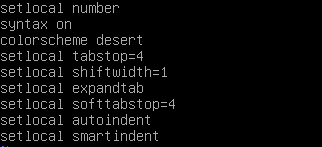
\includegraphics[width=\linewidth]{Images/Preamble/Preamble.PNG}
				\caption*{Las configuraciones para los archivos \texttt{.c}.}
			\end{subfigure}
		\end{figure}




















%Remove whitspace when done, for ease of work.
\end{document}